
How do we make the inferential leap from \emph{ad hoc} conventions formed through interaction with a single partner to \emph{global} conventions expected to be shared throughout a community?
Grounding collective convention formation in the individual learning mechanisms explored in the previous section requires an explicit \emph{theory of generalization} capturing how people transfer what they have learned from one partner to the next.
One influential theory is that speakers simply ignore the identity of different partners and update a single monolithic representation after every interaction \cite{steels_self-organizing_1995,barr_establishing_2004,young_evolution_2015}.
We call this a \emph{complete-pooling} theory because data from each partner is collapsed into an undifferentiated pool of evidence \cite{gelman2006data}. 
Complete-pooling models have been remarkably successful at predicting collective behavior on networks, but have typically been evaluated only in settings where anonymity is enforced. 
For example, \citeA{centola_spontaneous_2015} asked how large networks of participants coordinated on conventional names for novel faces.
On each trial, participants were paired with a random neighbor but were not informed of that neighbor's identity, or the total number of different possible neighbors. 

While complete-pooling may be appropriate for some everyday social interactions, such as coordinating with anonymous drivers on the highway, it is less tenable for everyday communicative settings.
Knowledge about a partner's identity is both available and relevant for conversation \cite{eckert_three_2012, davidson_nice_1986}.
Partner-specificity thus poses clear problems for complete-pooling theories but can be easily explained by another simple model, where agents maintain separate expectations about meaning for each partner.
We call this a \emph{no-pooling} model \cite<see>[which contrasted no-pooling and complete-pooling models]{SmithEtAl17_LanguageLearning}.
The problem with no-pooling is that agents are forced to start from scratch with each partner.
Community-level expectations never get off the ground.

In other words, complete-pooling and no-pooling models are \emph{prima facie} unable to explain partner-specific or community-level convention formation, respectively. 
CHAI is a hierarchical \emph{partial-pooling} account that offers a solution to this puzzle. 
We propose that beliefs about language have hierarchical structure.
That is, the meanings used by different partners are expected to be drawn from a shared community-wide distribution but are also allowed to differ from one another in systematic, partner-specific ways.
This structure provides an inductive pathway for abstract population-level expectations to be distilled from partner-specific experience.
The key predictions distinguishing our model thus concern the pattern of generalization across partners.
Experience with a single partner ought to be relatively uninformative about further partners, hence our partial-pooling account behaves much like a no-pooling model in predicting strong partner-specificity and discounting outliers \cite<see>[which explores this prediction in a developmental context]{dautriche2021}.
After interacting with multiple partners in a tight-knit community, however, speakers should become increasingly confident that labels are not simply idiosyncratic features of a particular partner's lexicon but are shared across the entire community, gradually transitioning to the behavior of a complete-pooling model.
In this section, we test this novel prediction in a networked communication game.
We then explicitly compare CHAI to complete-pooling and no-pooling variants that lesion the hierarchy, using only the top level or bottom level, to evaluate the contribution of each component.

\subsection{Model predictions: Simulation 2.1}

\begin{figure}[t]
\centering
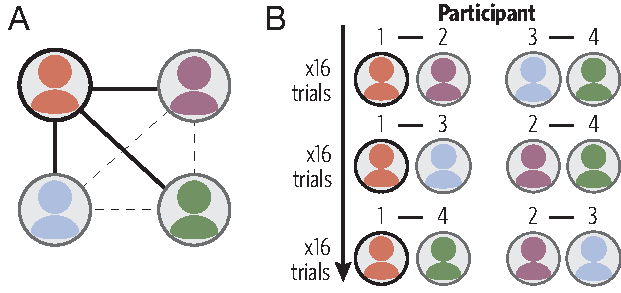
\includegraphics[scale=.8]{./figures/sec3-design.pdf}
\vspace{.1em}
\caption{In our simulations and behavioral experiment, participants were  (A) placed in fully-connected networks of 4, and (B) paired in a round-robin schedule of repeated reference games with each neighbor.}
\label{fig:task1_display}
\end{figure}

We first examine the generalization behavior produced by each model by simulating the outcomes of interacting with multiple partners on a small network (see Fig.~\ref{fig:task1_display}A). 
We used a round-robin scheme (Fig.~\ref{fig:task1_display}B) to schedule four agents into a series of repeated reference games with their three neighbors, playing 8 successive trials with one partner before advancing to the next, for a total of 24 trials.
These reference games used a set of two objects $\{o_1, o_2\}$ and four utterances $\{u_1, u_2, u_3, u_4\}$ as in Simulation 1.2; agents were randomized to roles when assigned to a new partner and swap roles after each repetition block within a given interaction.
Consequently, all agents at a particular phase have interacted with the same number of previous partners, allowing us to examine network convergence \cite<but see>[for a ``first-person'' version where each new partner is entirely fresh to the task, finding similar speaker generalization]{hawkins2020generalizing}.

Unlike our previous simulations with a single partner, where hierarchical generalization was irrelevant, we must now specify the hyper-prior P($\Theta$) governing the overall distribution of \emph{partners} (Eq.~\ref{eq:joint_inference}).
Following \citeA{KempPerforsTenenbaum07_HBM}, we extend the uniform categorical prior over possible referents to a hierarchical Dirichlet-Multinomial model \cite{gelman_bayesian_2014}, where the prior over the partner-specific meaning of $u$, $P(\phi_k(u_i)~=~o_j)$, is not uniform, but given by a parameter $\Theta$  that is shared across the entire population.
Because $\Theta$ is a vector of probabilities that must sum to 1 across referents, we assume it is drawn from a Dirichlet prior:
\begin{equation}
\label{eq:top_level}
\begin{array}{rcl}
\phi_k(u)  &\sim&  \textrm{Categorical}(\Theta) \\
\Theta & \sim & \textrm{Dirichlet}(\lambda \cdot \boldsymbol{\alpha})
\end{array}
\end{equation}
where $\lambda \cdot \boldsymbol{\alpha}$ gives the concentration parameter encoding the agent's beliefs, or ``over-hypotheses'' about both the central tendency and the variability of lexicons in the population. 
The relative values of the entries of $\boldsymbol{\alpha}$ correspond to inductive biases regarding the central tendency of lexicons, while the absolute magnitude of  the scaling factor $\lambda$ roughly corresponds to prior beliefs about the spread, where larger magnitudes correspond to more concentrated probability distributions across the population.
We fix $\lambda = 2$ and assume the agent has uncertainty about the population-level central tendency by placing a hyper-prior on $\alpha$ \cite<see>{cowans2004information} that roughly corresponds to the weak initial preferences we used in our previous simulations:
%We set $\boldsymbol{\alpha} = [1,1.5]$ for $u\in \{u_1,u_2\}$ and  $\boldsymbol{\alpha} = [1.5, 1]$ for $u\in\{u_3,u_4\}$ to encode weak initial preferences, as in Simulation 1.2.
\begin{figure*}[t]
\centering
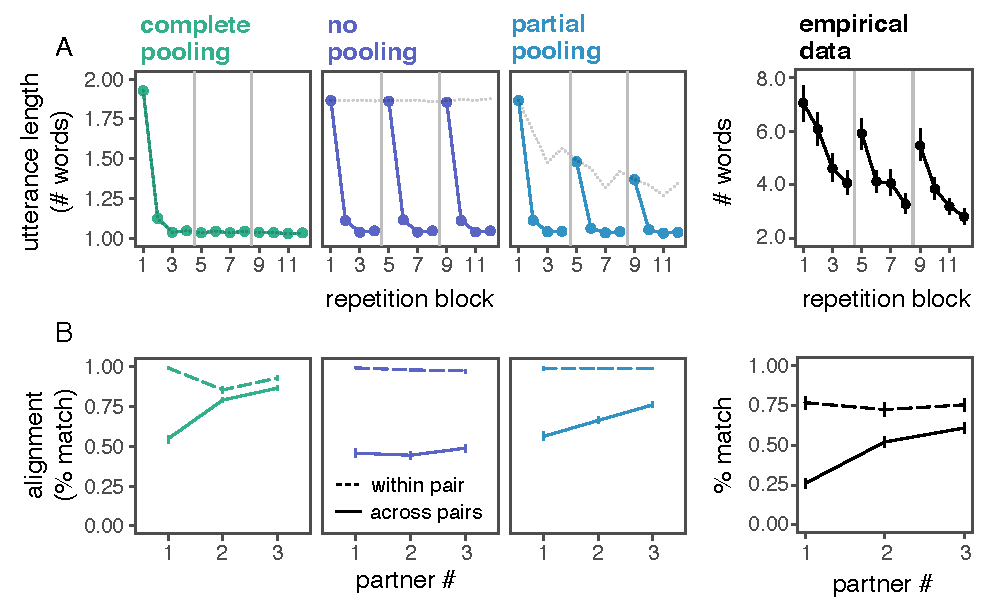
\includegraphics[scale=.8]{./figures/sec3-model-results.pdf}
\vspace{1em}
\caption{Simulation results and empirical data for (A) speaker reduction, and (B) network convergence across three partners. In (A) vertical boundaries mark time points when new partners were introduced, and the dotted grey line represents what would be produced for a stranger at each point in time. In (B), dashed line represents alignment between partners who are currently paired while solid line represents alignment across partners who are \emph{not} paired. Error bars represent bootstrapped 95\% confidence intervals.}
\label{fig:results}
\end{figure*}


\begin{equation*}
\begin{array}{rcl}
 \boldsymbol{\alpha} & \sim& \left\{
\begin{array}{rcl}
  \textrm{Dirichlet}(1.0,1.5)& \textrm{if} & u \in \{u_1, u_2\}\\
  \textrm{Dirichlet}(1.5,1.0) & \textrm{if} &u \in \{u_3, u_4\}\\
\end{array}\right. 
\end{array}
\end{equation*}

We may then define the no-pooling and complete-pooling models by lesioning this shared structure in different ways. 
The no-pooling model assumes an independent $\Theta_k$ for every partner, rather than sharing a single population-level parameter.
Conversely, the complete-pooling model assumes a single, shared $\phi$ rather than allowing different values $\phi_k$ for different partners.
We simulated 48 networks for each model, setting $\alpha_S = \alpha_L = 4,~w_C = .24$ (see Fig.~\ref{fig:partnerspecificity_grid} in the Appendix for an exploration of other parameters).

%For all simulations, we used variational inference as implemented in WebPPL \cite{GoodmanStuhlmuller14_DIPPL}
%Variational methods transform probabilistic inference problems into optimization problems by approximating the true posterior with a parameterized family.
%Specifically, we make a \emph{mean-field} approximation and assume that the full posterior can be factored into independent Gaussians for each random variable. 
%We then optimize the parameters of these posterior Gaussians by minimizing the evidence lower bound (ELBO) objective \cite<see>{murphy2012machine}.
%On each trial, we run 50,000 gradient steps on previous observations to obtain a posterior (Eq.\ 1) and compute the agent's marginal prediction for the next observation by taking the expectation over 50,000 samples from the variational guide (Eq. 4)\footnote{These details were chosen to ensure high-quality estimates of the model's behavior; see Discussion for other possible algorithms.}.

%\paragraph{Listener accuracy across partners}
%
%Next we consider the accuracy of a \emph{listener}'s expectations about which object is being referred to.
%The probability the listener assigns to the target on each trial is shown for the different models in Fig. \ref{fig:results}A.
%Under the partial-pooling model (top row), the listener model rapidly infers the meaning its partner is using and learns to choose the true target with higher accuracy after observing several trials of evidence from the same partner.
%When a second partner is introduced, the agent's expectations revert closer to their original state, unlike a complete-pooling model (second row).
%After observing multiple partners use utterances similarly, as the network converges, we find that this knowledge has gradually been incorporated into community-level expectations. 
%This is evident in much stronger initial expectations when introduced to the fourth partner ($\sim$ 75\% accuracy vs. 50\% with the first partner), unlike a no-pooling model (third row).
%
\paragraph{Speaker utterance length across partners}

We begin by examining our model's predictions about how a speaker's referring expressions change with successive listeners.
While it has been frequently observed that messages reduce in length across repetitions with a single partner \cite{krauss_changes_1964} and sharply revert back to longer utterances when a new partner is introduced \cite{wilkes-gibbs_coordinating_1992}, the key prediction distinguishing our model concerns behavior across subsequent partner boundaries.
Complete-pooling accounts predict no reversion in number of words when a new partner is introduced  (Fig.~\ref{fig:results}A, first column).
No-pooling accounts predict that roughly the same initial description length will re-occur with every subsequent interlocutor  (Fig.~\ref{fig:results}A, second column). 
% First, as in the complete-pooling and no-pooling models, we found that descriptions become more efficient over interaction with a single partner: the model becomes more confident that shorter utterances will be meaningful, so the marginal informativity provided by the longer utterance is not worth the additional cost.
%As in Simulation 1.2, we allowed a set of four primitive utterances, $\{u_1, u_2, u_3, u_4\}$, to be combined into conjunctions, e.g. $\{u_1u_2, u_3u_4, \dots\}$, which are assumed to have twice the utterance cost.
%The meanings of these conjunctions were determined compositionally from the values of the primitive utterances using a standard product T-norm for conjunction. 
%Again, we introduced a weakly biased prior for $\Theta$: two of the primitive utterances were expected to apply slightly more strongly to $o_1$ and the other two more strongly to $o_2$.
%Because our values come from a Gaussian prior and the T-norm is defined over $[0,1]$, we used logistic and logit function to map values to the unit interval and back.
%Speakers do not typically begin at chance over their \emph{entire} vocabulary,
%This weak bias leads to a preference for conjunctions at the outset and thus allows us examine reduction.

Here we show that a partial pooling account predicts a more complex pattern of generalization.
First, unlike the complete-pooling model, we find that the partial-pooling speaker model reverts or jumps back to a longer description at the first partner swap.
This reversion is due to ambiguity about whether the behavior of the first partner was idiosyncratic or attributable to community-level conventions.
In the absence of data from other partners, a partner-specific explanation is more parsimonious.
Second, unlike a no-pooling model, after interacting with several partners, the model becomes more confident that one of the short labels is shared across the entire community, and is correspondingly more likely to begin a new interaction with it (Fig.~\ref{fig:results}A, third column).

It is possible, however, that these two predictions only distinguish our partial-pooling model at a few parameter values; the no-pooling and complete-pooling could produce these qualitative effects elsewhere in parameter space.
To conduct a more systematic model comparison, then, we simulated 10 networks in each cell of a large grid manipulating the the optimality parameters $\alpha_S,\alpha_L$, the cost parameter $w_C$, and the memory discounting parameter $\beta$. 
We computed a ``reversion'' statistic (the magnitude of the change in $P(u_1u_2)$ immediately after a partner swap) and a ``generalization'' statistic (the magnitude of the change in $P(u_1u_2)$ from the initial trial with the agent's first partner to the initial trial with the final partner) and conducted single-sample $t$-tests at each parameter value to compare these statistics with what would be expected due to random variation.
We found that only the partial-pooling model consistently makes both predictions across a broad regime. 
The complete-pooling model fails to predict reversion nearly everywhere while the no-pooling model fails to predict generalization nearly everywhere.
Detailed results are shown in Fig.~\ref{fig:generalization_modelcomparison} in the Appendix.

\paragraph{Network convergence}

Because all agents are simultaneously making inferences about the others, the network as a whole faces a coordination problem.
For example, in the first block, agents 1 and 2 may coordinate on using $u_1$ to refer to $o_1$ while agent 3 and 4 coordinate on using $u_2$. 
Once they swap partners, they must negotiate this potential mismatch in usage. 
How does the network as a whole manage to coordinate?
We measured alignment by examining the intersection of utterances produced by speakers: if two agents produced overlapping utterances to refer to a given target (i.e.~a non-empty intersection), we assign a 1, otherwise we assign a 0.
We calculated alignment between currently interacting agents (i.e. \emph{within} a dyad) and those who were not interacting (i.e. \emph{across} dyads), averaging across the target objects.
Alignment across dyads was initially near chance, reflecting the arbitrariness of whether speakers reduce to $u_1$ or $u_2$. 
Under a complete-pooling model (Fig.~\ref{fig:results}B, first column), agents sometimes persist with mis-calibrated expectations learned from previous partners rather than adapting to their new partner, and \emph{within-dyad} alignment deteriorates, reflected by a sharp drop from 99\% to 85\%.
Under a no-pooling model (Fig.~\ref{fig:results}B, second column), convergence on subsequent blocks remains near chance, as conventions need to be re-negotiated from scratch.
By contrast, under our partial-pooling model, alignment across dyads increases without affecting alignment within dyads, suggesting that hierarchical inference leads to emergent consensus (Fig.~\ref{fig:results}B, third column).

\subsection{Behavioral experiment}

To evaluate the predictions derived in our simulations, we designed a natural-language communication experiment following roughly the same network design as our simulations.
That is, instead of anonymizing partners, as in many previous empirical studies of convention formation \cite<e.g.>{centola_spontaneous_2015}, we divided the experiment into blocks of extended dyadic interactions with stable, identifiable partners \cite<see>[for similar designs]{fay_interactive_2010, garrod_conversation_1994}.
Each block was a full repeated reference game, where participants had to coordinate on \emph{ad hoc} conventions for how to refer to novel objects with their partner.
Our partial-pooling model predicted that these conventions will partially reset at partner boundaries, but agents should be increasingly willing to transfer expectations from one partner to another.

\paragraph{Participants}

We recruited 92 participants from Amazon Mechanical Turk to play a series of interactive, natural-language reference games using the framework described in \citeA{Hawkins15_RealTimeWebExperiments}.

\paragraph{Stimuli and procedure}

Each participant was randomly assigned to one of 23 fully-connected networks with three other participants as their neighbors (Fig. \ref{fig:task1_display}A). 
Each network was then randomly assigned one of three distinct contexts containing abstract tangram stimuli taken from \cite{ClarkWilkesGibbs86_ReferringCollaborative}.
The experiment was structured into a series of three repeated reference games with different partners, using these same four stimuli as referents.
Partner pairings were determined by a round-robin schedule (Fig. \ref{fig:task1_display}B).
The trial sequence for each reference game was composed of four repetition blocks, where each target appeared once per block.
Participants were randomly assigned to speaker and listener roles and swapped roles on each block.
After completing sixteen trials with one partner, participants were introduced to their next partner and asked to play the game again. 
This process repeated until each participant had partnered with all three neighbors.
Because some pairs within the network took longer than others, we sent participants to a temporary waiting room if their next partner was not ready. 

Each trial proceeded as follows.
First, one of the four tangrams in the context was highlighted as the \emph{target object} for the speaker.
They were instructed to use a chatbox to communicate the identity of this object to their partner, the listener.
The two participants could engage freely in dialogue through the chatbox but the listener must ultimately make a selection from the array. 
Finally, both participants in a pair were given full feedback on each trial about their partner's choice and received bonus payment for each correct response. 
The order of the stimuli on the screen was randomized on every trial to prevent the use of spatial cues (e.g. ``the one on the left'').
The display also contained an avatar for the current partner  representing different partners with different colors as shown in Fig.~\ref{fig:task1_display} to emphasize that they were speaking to the same partner for an extended period.
On the waiting screen between partners, participants were shown the avatars of their previous partner and upcoming partner and told that they were about to interact with a new partner.

\subsection{Results}

We evaluated participants' generalization behavior on the same metrics we used in our simulations: utterance length and network convergence.

%\paragraph{Listener accuracy}
%
%We first examined changes in the proportion of correct listener selections.
%In particular, our partial pooling model predicts (1) gains in accuracy within each partner and (2) drops in accuracy at partner boundaries, but (3) overall improvement in initial interactions with successive partners.
%To test the first prediction, we constructed a logistic mixed-effects regression predicting trial-level listener responses. 
%We included a fixed effect of repetition block within partner (1, 2, 3, 4), along with random intercepts and slopes for each participant and each tangram. 
%We found that accuracy improved over successive repetitions with each partner, $b=0.69,z=3.87, p<0.001$.
%
%To test changes at partner boundaries, we constructed another regression model.
%We coded the repetition blocks immediately before and after each partner swap, and included this as a categorical fixed effect.
%Because partner roles were randomized for each game, the same participant often did not serve as listener in both blocks, so in addition to tangram-level intercepts, we included random slopes and intercepts at the \emph{network} level (instead of the participant level).
%We found that at the two partner swaps, accuracy dropped significantly, $b = -1.56, z = -2, p = 0.045$, reflecting the fact that the population has not completely converged on a shared system of meaning.
%Finally, to test whether performance improves for the \emph{very first} interaction with each new partner, before observing any partner-specific information, we examined the simple effect of partner number on the trials immediately after the partner swap (i.e. $t=\{1,5,9\}$).
%As predicted, we found a significant improvement in performance, $b = 0.57, z = 2.72, p = 0.007$, suggesting that listeners are bringing increasingly well-calibrated expectations into interactions with novel neighbors (see Fig.~\ref{fig:results}A, bottom row).
%
%\begin{figure*}
%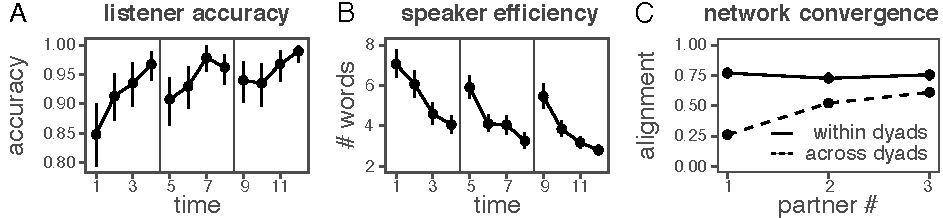
\includegraphics[scale=1.1]{./figures/sec3-empirical-results.pdf}
%\caption{Results from networked communication experiment. (A) Increase in accuracy across partners, (B) reduction in number of words across partners, (C) network convergence.}
%\label{fig:results}
%\end{figure*}


\paragraph{Speaker utterance length}

Now we are in a position to evaluate the central prediction of our model.
Our partial pooling model predicts (1) gains in efficiency within interactions with each partner and (2) reversions to longer utterances at partner boundaries, but (3) gradual shortening of  the initial utterance chosen with successive partners.
As a measure of efficiency, we calculated the raw length (in words) of the utterance produced on each trial.
Because the distribution of utterance lengths is heavy-tailed, we log-transformed these values.
To test the first prediction, we constructed a linear mixed-effects regression predicting trial-level speaker utterance length.
We included a fixed effect of repetition block within partner (1, 2, 3, 4), along with random intercepts and slopes for each participant and each tangram. 
We found that speakers reduced utterance length significantly over successive interactions with each individual partner, $b = -0.19,~t(34) = -9.88,~p < 0.001$.

To test the extent to which speakers revert to longer utterances at partner boundaries, we constructed another regression model.
We coded the repetition blocks immediately before and after each partner swap, and included it as a categorical fixed effect.
Because partner roles were randomized for each game, the same participant did not always serve as listener in both blocks, so in addition to tangram-level intercepts, we included random slopes and intercepts at the \emph{network} level (instead of the participant level).
As predicted, we found that utterance length increased significantly at the two partner swaps, $b = 0.43,~t(22) = 4.4,~p < 0.001$.

Finally, to test whether efficiency improves for the \emph{very first} interaction with each new partner, before observing any partner-specific information, we examined the simple effect of partner number at the trials immediately after the partner swap (i.e. $t=\{1,5,9\}$).
We found that participants gradually decreased the length of their initial descriptions with each new partner in their network, $b = -0.2,~t(516.5) = -6.07,~p < 0.001$ (see Fig. \ref{fig:results}A, final column), suggesting that speakers are bringing increasingly well-calibrated expectations into interactions with novel neighbors.
The partial-pooling model is the only model predicting all three of these effects.

\paragraph{Network convergence}

Now, we examine the \emph{content} of conventions and evaluate the extent to which alignment increased across the network over the three partner swaps. 
Specifically, we extend the same measure of alignment used in our simulations to natural language data by examining whether the intersection of words produced by different speakers was non-empty.
We excluded a list of common stop words (e.g. ``the'', ``both'') to focus on core conceptual content.
While this pure overlap measure provides a relatively weak notion of similarity, a more continuous measure based on the \emph{size} of the intersection or the string edit distance yielded similar results.

As in our simulation, the main comparison of interest was between currently interacting participants and participants who are not interacting: the partial-pooling model predicted that within-pair alignment should stay consistently high while (tacit) alignment between non-interacting pairs will increase. 
To test this prediction, we constructed a mixed-effects logistic regression including fixed effects of pair type (within vs. across), partner number, and their interaction.
We included random intercepts at the tangram level and maximal random effects at the network level (i.e. intercept, both main effects, and the interaction).
As predicted, we found a significant interaction ($b = -0.85, z = -5.69, p < 0.001$; see Fig. \ref{fig:results}B, final column).
Although different pairs in a network may initially use different labels, these labels begin to align over subsequent interactions. 

This finding is consistent with the primary prediction of interest for both the complete-pooling and partial-pooling model. %: (i.e. whether the partial-pooling model supports partner-specificity without interfering with network convergence). 
These two models only pull apart for a secondary prediction concerning the transition from the first to second partner.
The complete-pooling model predicts a significant drop in \emph{within-pair} convergence from the first to second partner, due to the continued influence of the first partner, while the partial-pooling model predicts no drop. 
We found no evidence of such a drop in the empirical data ($z=-0.66, p = 0.511$), providing further evidence in favor of the full partial-pooling structure.

\subsection{Discussion}

Drawing on general principles of hierarchical Bayesian inference, CHAI suggests that conventions represent the shared structure that agents ``abstract away'' from partner-specific learning.
In this section, we evaluated the extent to which CHAI captured human generalization behavior in a natural-language communication experiment on small networks.
Unlike complete-pooling accounts, it allows for partner-specific common ground to override community-wide expectations given sufficient experience with a partner, or in the absence of strong conventions.
Unlike no-pooling accounts, it results in networks that are able to converge on shared conventions.

Partner-specificity and generalization presents an even steeper challenge for previous accounts than \textbf{P1}. 
It is not straightforward for previous interactive alignment or reinforcement learning accounts to explain patterns across partner boundaries without being augmented with additional social information.
If a particular semantic representation has been primed due to precedent in the preceding dialogue, then the shifting identity of the speaker should not necessarily alter its influence \cite{brennan2009partner,ferreira2012priming,ostrand2019repeat}. 
More sophisticated hierarchical memory retrieval accounts that represent different partners as different \emph{contexts} \cite<e.g>{polyn2009context,BrownSchmidtEtAl15_Contexts} may allow priming to be modulated in a partner-specific way, but such an account would presuppose that social information like partner identity is already a salient and relevant feature of the communicative environment.
Indeed, an  account assuming socially-aware context reinstatement for partner-specific episodic memories, and slower consolidation of shared features into population-level expectations, may be one possible process-level candidate for realizing our hierarchical computational-level model.

A frequent concern in prior work using repeated reference games is that improvements in communication over time are due to generic effects of task familiarity and repetition rather than interactive adaptation to a partner's language use \cite{HupetChantraine92_CollaborationOrRepitition}. As they get more practice with the task, speakers may simply get better overall at describing images and listeners may learn how to better identify target images. The effects we observe at partner boundaries show that something is being learned beyond pure familiarity with the task: if speakers and listeners were just learning to better describe and identify targets regardless of who their partner is, we would not expect these reversions. These partner-specificity effects clearly rule out the complete pooling model, but cannot rule out a no-pooling model combined with a practice effect. Under this  alternative possibility, partner-specific adaptation would be genuine, but the general decrease in utterance length and increase in accuracy with new partners would be due to practice rather than inductive generalization.
Our best current evidence against this practice-based explanation lies in our network convergence results: networks as a whole converge to similar short descriptions across partners, and different networks converge to different descriptions, indicating some gradual degree of transfer across partners. 
Future work may further address these concerns by including filler trials or by manipulating the length of interaction with each partner.

Our account also predicts that similar inductive learning mechanisms would operate not only across different partners but across different contexts containing different referents. 
By holding the partner constant across different contexts, rather than holding the context constant across different partners, it would be possible to test the extent to which additional experience along one axis of generalization would affect generalization along the other axis. 
Finally, one subtler point, which we believe is a rich direction for future research, is how generalization may still depend on the speaker’s beliefs about \emph{how partners are sampled}, manifested in their inductive biases at the community-level (Eq.~\ref{eq:top_level}).
If they believe they are in a tight-knit community where different partners are experts with the domain and have likely interacted with one another before, they may generalize differently than if they believe their community has higher turnover and many novices, brand-new to the task \cite{isaacs_references_1987}.

%While our behavioral data appears inconsistent with complete-pooling and no-pooling accounts, there remain deep theoretical connections between our hierarchical Bayesian formulation and alternative theories of generalization which may also be considered ``partial-pooling'' \cite{rogers2004semantic,marcus2018algebraic,doumas2008theory}.
%For example, recent neural network algorithms such as Model-Agnostic Meta-Learning \cite<MAML>{FinnAbeelLevine17_MAML}, which attempt to learn general parameter settings (e.g. conventions) that can rapidly adapt to different specific tasks (e.g. partners), have been shown to be equivalent to hierarchical Bayes under certain conditions \cite{grant_recasting_2018}.
%Such neural network instantiations may scale better in practice to natural language in more complex referential spaces, and may only require a handful of gradient steps to successfully adapt \cite{hawkins2019continual}.
%Alternatively, if different partners are represented as different contexts \cite{brown2015people}, then appropriately hierarchical reinforcement learning mechanisms may produce similar predictions \cite{gershman2015novelty}.
%These theoretical connections expose a common underlying view that conventions emerge from a group of agents discovering latent structure in coordination problems by adapting to each idiosyncratic partner along the way.
